\documentclass{beamer}   % [notes=show,handout]

\usepackage{tikz}
\usepackage{graphicx}
\mode<presentation>

\usetheme{Frankfurt}%
\usecolortheme{seagull}

\definecolor{garnet}{RGB}{136,0,0}
\definecolor{clarksonGreen}{RGB}{0,52,21}

\setbeamercolor{palette primary}{fg=garnet,bg=white}
\setbeamercolor{palette secondary}{fg=clarksonGreen,bg=white}
\setbeamercolor{palette tertiary}{fg=clarksonGreen,bg=white}
\setbeamercolor{palette quaternary}{bg=clarksonGreen,fg=white}
\setbeamercolor{block title}{fg=black,bg=black!15}
\setbeamercolor{block body}{fg=black,bg=black!10}
\setbeamercolor{titlelike}{bg=garnet,fg=white} % parent=palette quaternar

\setbeamertemplate{footline}{\hspace*{.5cm}\scriptsize{\insertauthor
\hspace*{50pt} \hfill\insertframenumber\text{/}\inserttotalframenumber\hspace*{.5cm}}}

\newcommand{\R}{\mathbb{R}}


\begin{document}



\part{Introduction}
\lecture{Introduction}{Introduction}


\title{Stochastic Differential Equations}
\subtitle{Midterm Presentation}

\author{Liu, Sweeney, Zhou}
\institute{SUNY Potsdam and Clarkson University REU \\ with Dr. Kelly Black}
\date{July 5, 2013}

\begin{frame}[plain]
  \titlepage
  \begin{center}
  
\includegraphics[width=0.2\textwidth]{SUNYPotsdam}
  
\includegraphics[width=0.1\textwidth]{nsf_logobig}
  
\includegraphics[width=0.15\textwidth]{clarksonGreen}
\end{center}
\end{frame}

\begin{frame}
  \frametitle{Outline}
  \vspace{-5mm}
  \tableofcontents[pausesection,hideallsubsections]
\end{frame}



\section{Brownian Motion}


\begin{frame}
    \frametitle{Distribution and Limit Process}
	\begin{center}
		$Y_{n} = X_{0}+ X_{1}+X_{2}+...+X_{n}$
	\end{center}
	\begin{itemize}
		\item Characteristic Function
			\begin{eqnarray}
				E[e^{itY_{n}}]&=& \cos(t\triangle x)^{\frac{T}{\triangle t}}\\
				\lim_{n\rightarrow \infty} E[e^{itY_{n}}]&=& e^{\frac{-\lambda^{2} T}{2}} \label{eqn:limwalk}
			\end{eqnarray}
		\item Equation (\ref{eqn:limwalk}) implies that $ \lim_{n\rightarrow \infty} Y_{n} \sim $N(0, T)			
	\end{itemize}

\end{frame}

%%%%%%%%%%%%%%%%%%% Property 3
\begin{frame}
    \frametitle{Brownian Motion}
Properties
	\begin{enumerate}[i]
		\item $B(t)$ is continuous
		\item $B(t)$ is no where differentiable
		\item If $t_{1}<t_{2}<t_{3}<t_{4}$, \\
			$B(t_{1}), B(t_{2})-B(t_{1}),  B(t_{3})-B(t_{4})$ are independent random variables
		\item If $0 \le s\le t$ then $B(t)-B(s) \sim N(0, t-s)$
	\end{enumerate}
\end{frame}











\section{Stochastic Integral}
%%%%%%%%%% ai left
\begin{frame}
    \frametitle{Characteristic Functions and Step Functions}
	\begin{eqnarray}
	1_{[t_{i-1}, t_{t})}(t) &=& \left\{\begin{matrix}
	1 &  if \ t_{i-1} \le t < t_{i}\\ 
	0 &  otherwise
	\end{matrix}\right.
	\end{eqnarray}

	\begin{eqnarray}
		f_{n}(t) &=& \sum_{i=1}^{n} a_{i} 1_{ [t_{i-1} , t_{t} ) }(t)
	\end{eqnarray}

\end{frame}




\begin{frame}
    \frametitle{Stochastic Integral}
	\begin{eqnarray*}
		I(f_{n})&=&\int_{a}^{b}f_{n}(t)\,dB = \sum_{i=1}^{n} a_{i}[B(t_{i})-B(t_{i-1})]	
	\end{eqnarray*}
\begin{itemize}
		\item $I(f_{n}(t))$ is a normally distributed random variable
		\item E[$I(f_{n}(t))$] = 0
		\item Var[$I(f_{n}(t))$] = $\int^b_a f_{n}^{2} (t)\,dt$
	\end{itemize}


\end{frame}

\begin{frame}
    \frametitle{Riemann-Stieltjes Stochastic Integration}
	\begin{eqnarray*}
		\int^b_a  f(t) \, dB(t) &=&  f(t)B(t) \, \bigg|_{a}^{b} -  \left( \mathrm{RS} \right) 			\int^b_a B(t)\,df(t)		
	\end{eqnarray*}

\end{frame}









\section{It\^{o}'s Formula}

\begin{frame}
    \frametitle{Second Order Taylor Expansion}
	\begin{eqnarray}
		f(t,x)-f(a,x_{0}) &=& \frac{\partial f}{\partial t}(a,x_{0})(t-a) + \frac{\partial f}{\partial x}(a,x_{0})(x-x_{0}) +\nonumber \\  
		&& \frac{\partial^{2}f}{\partial t^2}(a,x_{0})\frac{1}{2!}(t-a)^{2} +\nonumber \\  
		&&\frac{\partial^{2}f}{\partial t \partial x}(a,x_{0})(t-a)(x-x_{0}) +\nonumber \\  
		&&\frac{\partial^{2}f}{\partial x^{2}}(a,x_{0})\frac{1}{2!}(x-x_{0})^{2}+\mathrm{H.O.T.}.
	\end{eqnarray}

\end{frame}

\begin{frame}
    \frametitle{Second Order Taylor Expansion}
	\begin{eqnarray}
		f(t,B(t))-f(a,B(a)) &=& \frac{\partial f}{\partial t}(a,B(a))(t-a) + \nonumber \\ 
		&&\frac{\partial f}{\partial B}(a,B(a))(B(t)-B(a)) +\nonumber \\  
		&& \frac{\partial^{2}f}{\partial t^2}(a,B(a))\frac{1}{2!}(t-a)^{2} +\nonumber \\  
		&&\frac{\partial^{2}f}{\partial t \partial B}(a,B(a))(t-a)(B(t)-B(a)) +\nonumber \\  
		&&\frac{\partial^{2}f}{\partial B^{2}}(a,B(a))\frac{1}{2!}(B(t)-B(a))^{2}+\nonumber \\ 
		&&\mathrm{H.O.T.}.
	\end{eqnarray}

\end{frame}

\begin{frame}
    \frametitle{It\^{o}'s Formula}

	\begin{eqnarray}
		f(t, B(t))-f(a, B(a)) &=&\int^t_a \frac{\partial f}{\partial s}(s, B(s)) + \frac{1}{2} 			\frac{\partial^{2} f}{\partial B^{2}}(s, B(s)) \, ds \nonumber \\  
		&&+\int^t_a \frac{\partial f}{\partial B}(s, B(s)) \, dB 
	\end{eqnarray}

\end{frame}








\section[SDE]{Stochastic Differential Equations}

\begin{frame}
    \frametitle{Ordinary Differential Equation}
	\begin{eqnarray*}	
	X(t) &=& X(0) + \int^t_0 g(x,s)\,ds,
	\end{eqnarray*}
	\begin{eqnarray*}
	dX(t)&=&g(x,t)dt. 
	%%% Physical meaning? dB , ds
	\end{eqnarray*}

\end{frame}

\begin{frame}
    \frametitle{Stochastic Differential Equation}
	\begin{eqnarray*}	
	X(t) &=& X(0) + \int^t_0 f(x,s)\,dB(s) + \int^t_0 g(x,s)\,ds,
	\end{eqnarray*}
	\begin{eqnarray*}
	dX(t)&=&f(x,t)\,dB(t)+g(x,t)\,dt. 
	%%% Physical meaning? dB , ds
	\end{eqnarray*}

\end{frame}

\begin{frame}
    \frametitle{Exponential Decay}
	\begin{eqnarray*}
		dX(t) &=& -\beta X(t)\,dt,
	\end{eqnarray*}
	\begin{eqnarray*}
		X(t) &=& X(0)e^{-\beta t}.
	\end{eqnarray*}

\end{frame}


\begin{frame}
    \frametitle{Langevin Stochastic Differential Equation (Additive Noise)}
	%%% Mention constant additive noise
	\begin{eqnarray*}
		dX(t) &=& \alpha\,dB(t)-\beta X(t)\,dt,		
	\end{eqnarray*}
	\begin{eqnarray*}
		X(t)&=& X(0) e^{- \beta t} + \alpha e^{- \beta t} \int^t_0 e^{\beta s} \, dB(s).
	\end{eqnarray*}
\end{frame}


\begin{frame}
    \frametitle{Geometric Brownian Motion (Multiplicative Noise)}
	%%% Mention multiplicative noise
	%%% Dependent on the amount of stuff - higher price more fluctuations
	\begin{eqnarray*}
		dX(t) &=& \alpha X(t) \, dB(t)-\beta X(t) \, dt, 
	\end{eqnarray*}
	\begin{eqnarray*}
		X(t) &=& X(0)e^{\alpha B(t) - (\beta + \frac{1}{2} \alpha^{2})t}.			
	\end{eqnarray*}

\end{frame}







\section{Numerical Simulations}
%%%%% Reviewing
\begin{frame}
    \frametitle{Random Walk Positions}
    \hspace{-7mm}
    \vspace{4mm}
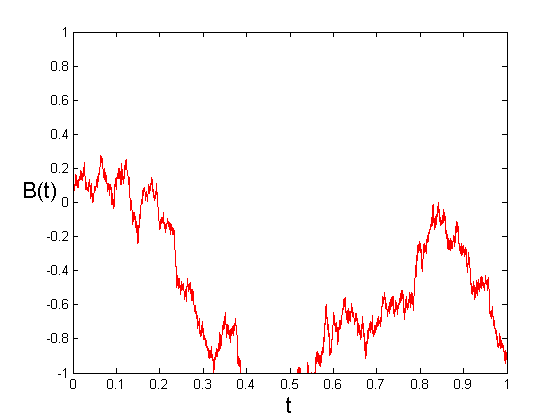
\includegraphics[height=6cm,width=6cm]{rw1}
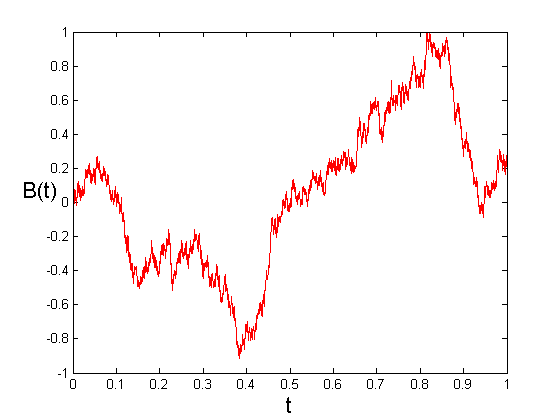
\includegraphics[height=6cm,width=6cm]{rw2}
\end{frame}

\begin{frame}
    \frametitle{Random Walk Positions}
    \hspace{-7mm}
    \vspace{4mm}
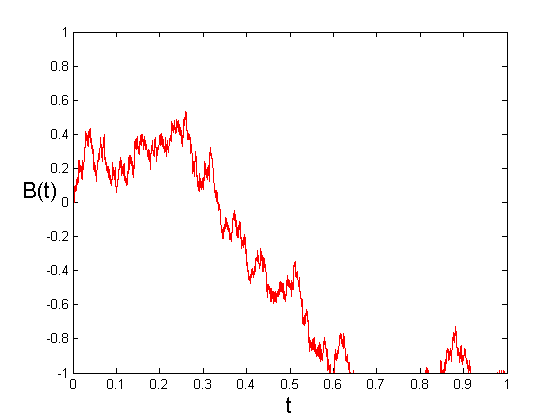
\includegraphics[height=6cm,width=6cm]{rw3}
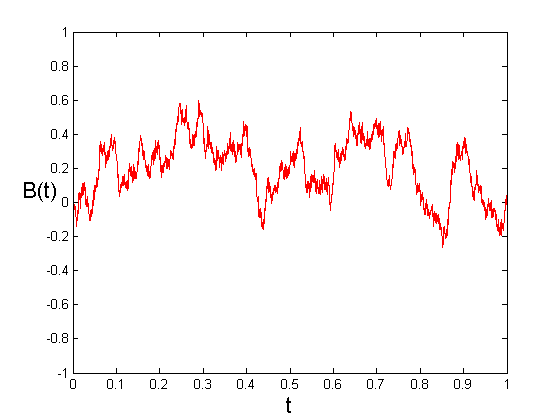
\includegraphics[height=6cm,width=6cm]{rw4}
\end{frame}

\begin{frame}
    \frametitle{Random Walks Distribution}
    \hspace{-5mm}
    \vspace{4mm}
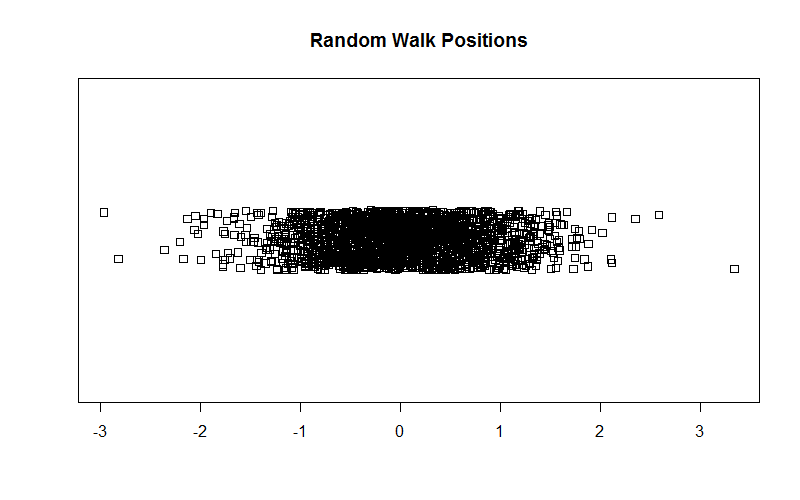
\includegraphics[height=7cm,width=6cm]{rw_jitter}
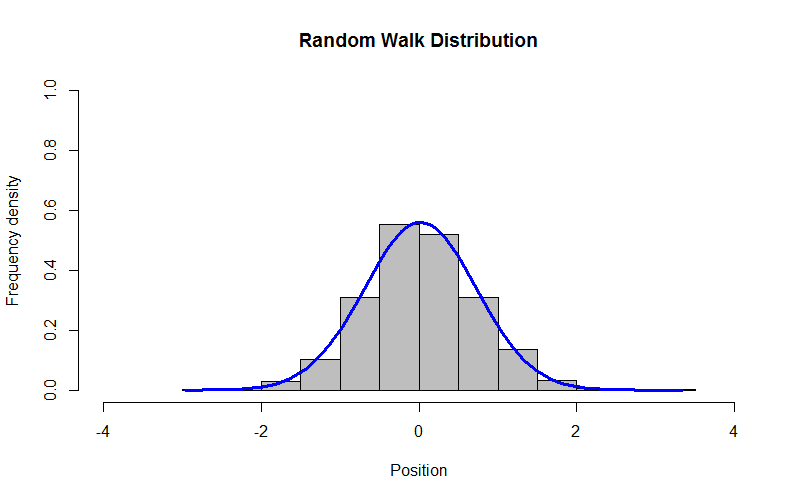
\includegraphics[height=7cm,width=6cm]{rw_hist}
\end{frame}



\begin{frame}
    \frametitle{Stochastic Integrals}
    \vspace{-7mm}
    \hspace{-6mm}
	\begin{eqnarray*}
		\int^t_0 B(s)\,dB(s) &=& \frac{1}{2}B^{2}(t)-\frac{1}{2}t		
	\end{eqnarray*}
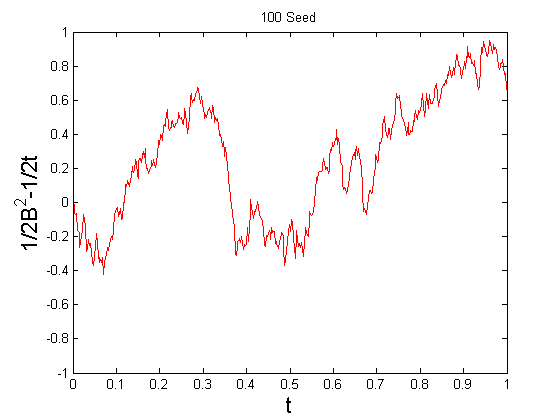
\includegraphics[height=6cm,width=6cm]{wdw_100}
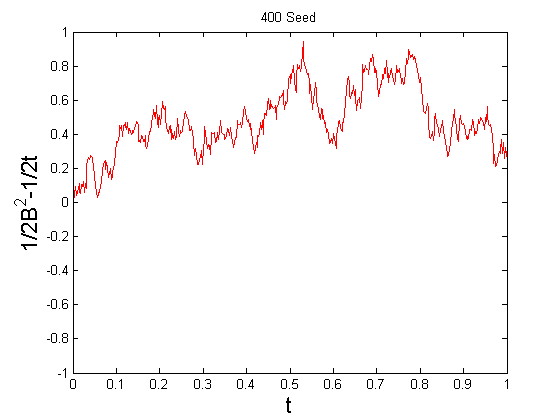
\includegraphics[height=6cm,width=6cm]{wdw_400} 
\end{frame}


\begin{frame}
    \frametitle{Exponential Functions of $B(t)$}
    \hspace{-5mm}
    \vspace{4mm}
	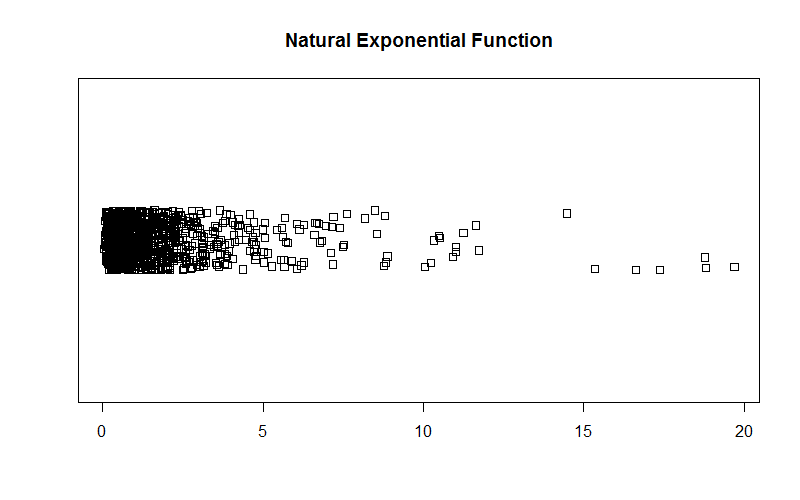
\includegraphics[height=7cm,width=6cm]{expB_jitter}
	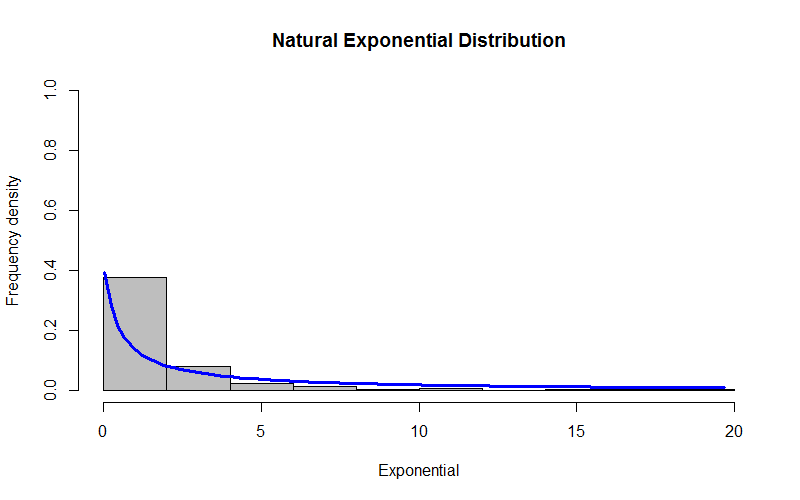
\includegraphics[height=7cm,width=6cm]{expB_hist} 
\end{frame}



\begin{frame}
    \frametitle{Euler-Maruyama Method vs Milstein Method}
    \vspace{-10mm}
  	\begin{eqnarray*}
	dX(t)&=&f(x,t)dB(t)+g(x,t)dt. 
	\end{eqnarray*} 
     \begin{definition}[Euler-Maruyama Method]
    \begin{eqnarray*}
		X_{j} &=& X_{j-1} + f(X_{j-1})\triangle t+ g(X_{j-1})(W(\tau_{j})-W(\tau_{j-1}))
		\\ j &=& 1,2,... ,L	
\end{eqnarray*}
\end{definition}
\begin{definition}[Milstein Method]
	\begin{eqnarray*}
		X_{j} &=& X_{j-1} + \triangle tf(X_{j-1}) + g(X_{j-1})(W(\tau_{j})-W(\tau_{j-1})) 			\nonumber\\ 
		&& + \frac{1}{2} g(X_{j-1})g'(X_{j-1})((W(\tau_{j})-W(\tau_{j-1}))^{2}-\triangle t)
		\\ j &=& 1,2,... ,L
	\end{eqnarray*}
\end{definition}
\end{frame}

\begin{frame}
  \frametitle{Euler-Maruyama Method vs Milstein Method}
  \vspace{-10mm}	
  \begin{eqnarray*}
		dX(t) &=&  X(t) \,dB(t)+ 2 X(t) \,dt
\end{eqnarray*}
%%%%% so alpha=1 and beta = -2 (exponential growtn not decay)
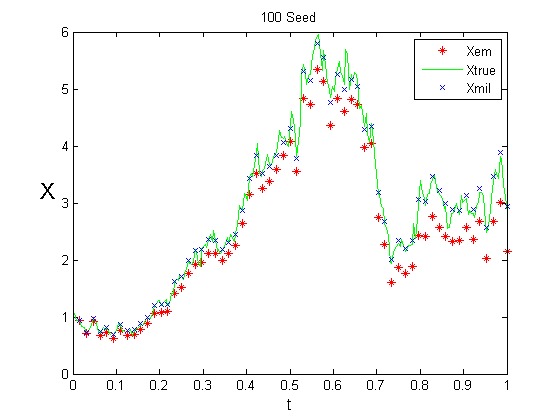
\includegraphics[height=5cm,width=6cm]{emmil_seed100}
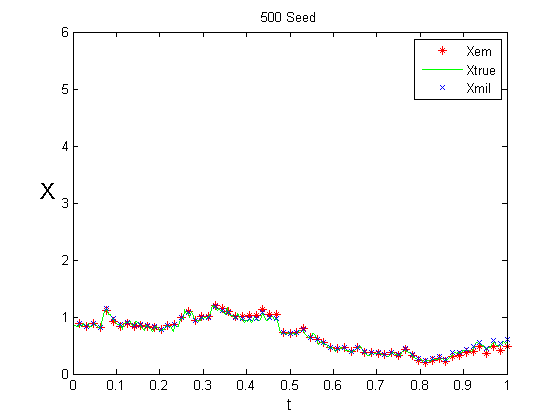
\includegraphics[height=5cm,width=6cm]{emmil_seed500}
\end{frame}


\begin{frame}
    \frametitle{Euler-Maruyama Method vs Milstein Method}
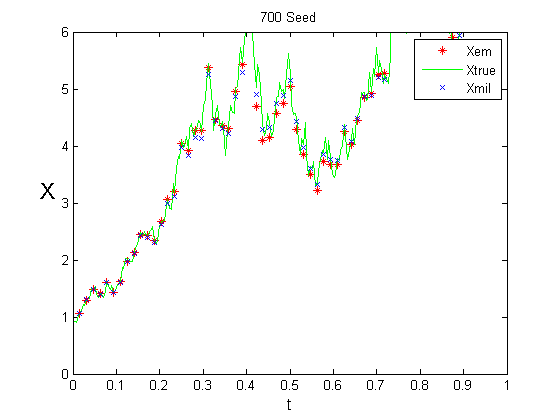
\includegraphics[height=5cm,width=6cm]{emmil_seed700}
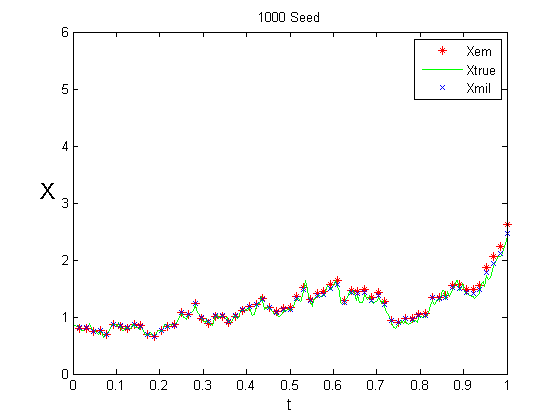
\includegraphics[height=5cm,width=6cm]{emmil_seed1000}
\end{frame}




%\section{Financial Applications}

%\begin{frame}
    %\frametitle{American Option vs European Option \\ \&  Call vs Put}
	%\begin{itemize}
	%	\item American Option - Option that can only be exercised at its maturity
	%	\item European Option -  Option that can be exercised anytime during its life 
	%	\item Call - Option to buy at a certain price
	%	\item Put - Option to sell at a certain price
	%\end{itemize}		
% \end{frame}





\section{Possible Goals/Questions?}

\begin{frame}
    \frametitle{Possible Goals/Questions?}
	\begin{itemize}
		\item Actuarial Applications
		\item An evaluation of a mitigation strategy for deer-vehicle collisions (Bissonette, Rosa, 2012)
		\item Designing Index-Based Livestock Insurance for Managaing Asset Risk in Northern Kenya (Chantarat, \emph{et al.}, 2013) 
	\end{itemize}
\end{frame}


\begin{frame}
    \frametitle{Acknowledgements}
	Thanks to Dr. Joel Foisy, Dr. Kelly Black and NSF (NSF\#1262737) for their support and involvement in this program.
\end{frame}




\end{document}